\let\negmedspace\undefined
\let\negthickspace\undefined
\documentclass[journal]{article}
\usepackage[a5paper, margin=10mm, onecolumn]{geometry}
\usepackage{lmodern} % Ensure lmodern is loaded for pdflatex

\setlength{\headheight}{1cm} % Set the height of the header box
\setlength{\headsep}{0mm}     % Set the distance between the header box and the top of the text

\usepackage{gvv-book}
\usepackage{gvv}
\usepackage{cite}
\usepackage{amsmath,amssymb,amsfonts,amsthm}
\usepackage{algorithmic}
\usepackage{graphicx}
\graphicspath{{./figs/}}
\usepackage{textcomp}
\usepackage{xcolor}
\usepackage{txfonts}
\usepackage{listings}
\usepackage{enumitem}
\usepackage{mathtools}
\usepackage{gensymb}
\usepackage{comment}
\usepackage[breaklinks=true]{hyperref}
\usepackage{tkz-euclide} 
\usepackage{listings}
\usepackage{gvv}                                        
\def\inputGnumericTable{}                                 
\usepackage[latin1]{inputenc}                                
\usepackage{color}                                            
\usepackage{array}                                            
\usepackage{longtable}                                       
\usepackage{calc}                                             
\usepackage{multirow}                                         
\usepackage{hhline}                                           
\usepackage{ifthen}                                           
\usepackage{lscape}
\usepackage{circuitikz}
\tikzstyle{block} = [rectangle, draw, fill=blue!20, 
text width=4em, text centered, rounded corners, minimum height=3em]
\tikzstyle{sum} = [draw, fill=blue!10, circle, minimum size=1cm, node distance=1.5cm]
\tikzstyle{input} = [coordinate]
\tikzstyle{output} = [coordinate]


\begin{document}
	
	\bibliographystyle{IEEEtran}
	\vspace{3cm}
	
\title{1.5.34}
\author{EE25BTECH11047 - RAVULA SHASHANK REDDY}
\maketitle
\hrulefill
\bigskip 

\renewcommand{\thetable}{\theenumi}
\setlength{\intextsep}{10pt}

\textbf{Question}:\\

The point \(P\) which divides the line segment joining the points \(A(2,-5)\) and \(B(5,2)\) in the ratio \(2:3\) lies in which quadrant?\\

\textbf{Solution}:\\

  Given:
\begin{align}
\vec{A} = \myvec{2 \\ -5} \\ \vec{B} = \myvec{5 \\ 2}
\end{align}

Now the matrix form for $\vec{A}$ and $\vec{B}$ is :
\begin{align}
    \myvec{\vec{A} & \vec{B}} = \myvec{2 & 5 \\ -5 & 2}
\end{align}
The point \(P\) dividing the segment \(AB\) in the ratio 2:3 internally , has the position vector :
\begin{align}
\vec{P} = \frac{ 3\vec{A} +2\vec{B} }{3+2} 
\end{align}
Thus by using the section formula \\
\begin{align} 
\vec{P}= \frac{1}{5} \cdot \myvec{\vec{A} & \vec{B}}\myvec{3 \\ 2}\\
\vec{P}= \frac{1}{5} \cdot \myvec{2 & 5 \\ -5 & 2}\myvec{3 \\ 2}\\
\vec{P}= \frac{1}{5} \cdot \myvec{6 + 10\\ -15 + 4}\\
\therefore \vec{P}= \frac{\myvec{16 \\ -11}}{5}.
\end{align}

Hence the vector $\vec{P}$ is \myvec{\frac{16}{5} \\ \frac{-11}{5}}  = \myvec{3.2 \\ -2.2} \\[4pt]
Since \(x>0\) and \(y<0\), $\vec{P}$ lies in the \textbf{IV (fourth) quadrant}.
\newpage
\begin{figure}
    \centering
    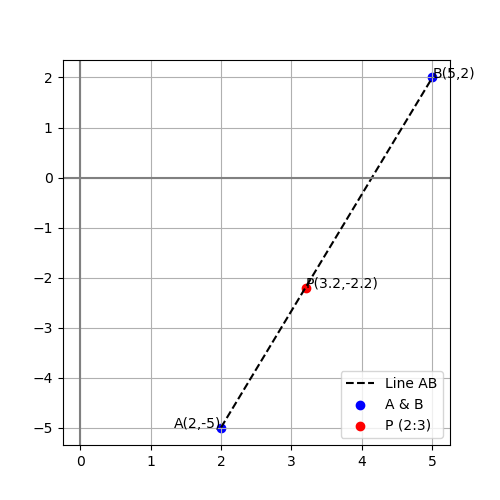
\includegraphics[width=0.9\linewidth]{figs/fig_1.png}
    \caption{}
    \label{fig:placeholder}
\end{figure}
\begin{figure}
    \centering
    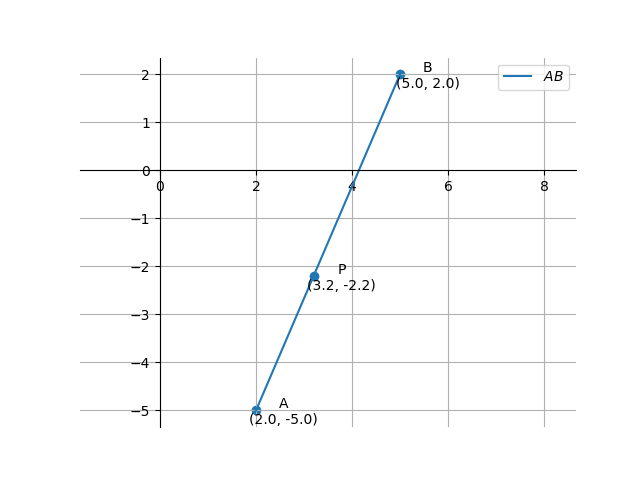
\includegraphics[width=1.0\linewidth]{figs/fig_2.png}
    \caption{}
    \label{fig:placeholder}
\end{figure}
\end{document}